\chapter{Machine Learning}
\section{Introduction}

Machine learning, a subfield of artificial intelligence, is a scientific discipline that focuses on the development of algorithms and statistical models that enable computers to carry out specific tasks by learning patterns from data. It involves the creation of models that can be supervised (learning from labeled data), unsupervised (learning from unlabeled data), semi-supervised, or with reinforcement (learning based on reward/punishment system). Machine learning has a wide range of applications, including but not limited to, natural language processing, image recognition, and recommendation systems \cite{mitchell1997machine}.

Within the framework of the JUNO experiment, machine learning algorithms are utilized to analyze the data, discerning patterns that represent IBD events, thereby effectively differentiating them from the background.

\subsection{Supervised Learning}
Supervised learning is a fundamental aspect of machine learning, where algorithms are trained using labeled datasets. In this approach, the algorithm learns from examples that are already labeled with the correct answers. The goal is to develop a function that accurately maps input data to corresponding outputs.
In the context of this thesis, the focus is on binary classification in the JUNO experiment. The objective is to classify a given event pair as either a correlated inverse event pair or an accidental background event pair, utilizing the event pair's features.

Two different machine learning algorithms, \textbf{Boosted Decision Trees} (BDT) and \textbf{Neural Network} (NN), are deployed to  to perform the classification task.

\section{Boosted Decision Trees}

Gradient Boosting is a machine learning technique that leverages the concept of boosting, combined with the methodology of gradient descent. The objective is to construct a robust predictive model by amalgamating multiple weak learners, which are typically decision trees \cite{gb_1}.

The unique aspect of Gradient Boosting, compared to traditional boosting techniques, is its method of error correction. Rather than altering the weights of misclassified instances, the model fits each subsequent tree to the residuals (or the negative gradient) of the loss function relative to the prediction of the existing ensemble of trees. This implies that each new tree is trained to predict the error of the current model, thereby progressively reducing the overall error.

The process is formalized as follows:

\begin{enumerate}
    \item \textbf{Initialization}: The model is initiated with a constant value, denoted as 
    \begin{equation*}
        F_0(x) = \arg\min_{\gamma} \sum_{i=1}^{N} L(y_i, \gamma)    
    \end{equation*}
    where $L(y, F(x))$ represents the loss function, $y$ is the true target value, and $F(x)$ is the model's prediction for the input features $x$. This constant prediction, $\gamma$, is chosen to minimize the total loss over all $N$ instances.

    \item \textbf{Computation of Residuals}: The model iteratively constructs an ensemble of $M$ trees. For each iteration $m=1$ to $M$, the residuals are calculated as 
    \begin{equation*}
        r_{im} = - \left[\frac{\partial L(y_i, F(x_i))}{\partial F(x_i)}\right]_{F(x)=F_{m-1}(x)}
    \end{equation*}
     for each instance $i=1,2,...,N$. These residuals are essentially the negative gradients of the loss function with respect to the model's predictions
     
   \item \textbf{Fitting a Decision Tree}: After computing the residuals, we fit a new decision tree, $h_m(x)$, to these residuals. This tree is thus trained to predict the negative gradient of the loss function, using the training set ${(x_i, r_{im})}_{i=1}^n$. By doing so, it attempts to correct the errors made by the current ensemble model.
	
    \item \textbf{Model Update}: The model is then updated by applying the rule
    \begin{equation*}
        F_m(x) = F_{m-1}(x) + \nu \cdot h_m(x)
    \end{equation*}
    Here, $\nu$ represents the learning rate, a parameter typically less than 1, which controls the contribution of each tree to the final prediction.	

    \item \textbf{Final Model}: The final model's prediction is given by
    \begin{equation*}
        F_M(x) = F_0(x) + \sum_{m=1}^{M} \nu \cdot h_m(x)
    \end{equation*}
    In the final ensemble model, each decision tree provides a correction to the predictions of the previous trees, collaboratively reducing the loss function's value and improving the overall model's performance \cite{gb_1}.
\end{enumerate}

XGBoost is an highly efficient implementation of this method, which introduces several improvements such as parallel processing \cite{gb_2}.



\section{Neural Networks}
Neural Networks (NNs) are computational models that draw inspiration from the interconnected structure of the human brain \cite{haykin2009neural}. 

An artificial neuron takes inputs $ x = [x_1, x_2, ..., x_n] $, applies weights $ w = [w_1, w_2, ..., w_n] $ to the inputs, sums them, and adds a bias term $ b $. Mathematically, this operation can be represented as:

\[
z = \sum_{i=1}^{n} w_i x_i + b 
\]

The calculated value, $ z $, is then passed through an \textit{activation function}, $ f $, to generate the neuron's output, $ a = f(z) $ \cite{haykin2009neural}.

The activation function introduces non-linearity into the model, which is crucial for the network's ability to learn complex patterns. Common choices for $ f $ include the sigmoid, hyperbolic tangent, and ReLU (Rectified Linear Unit) functions \cite{goodfellow2016deep}.

An Artificial Neural Network (ANN) consists of interconnected layers of neurons, including an input layer, one or more hidden layers, and an output layer. Each layer is fully connected to the next layer. A graphical representation of an Artificial Neural Network and a single neuron is presented in Figure \ref{fig:nn} and Figure \ref{fig:neuron} \cite{goodfellow2016deep}.

 
%TODO: Migliorare la qualità dell imagine, eliminare la parte scritta

\begin{figure}[h!]
	\centering
	
	\subfloat[Graphic representation of ANN]{
		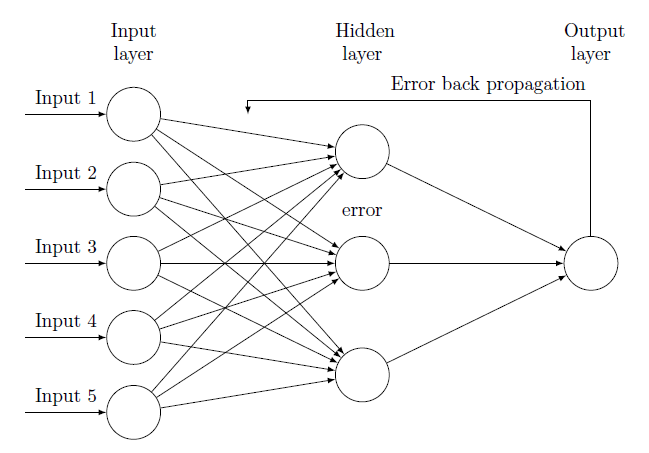
\includegraphics[width = 0.4\textwidth]{Images/fig_neural_network}
		\label{fig:nn}
	}
	\centering
	\subfloat[Single Neuron representation]{
		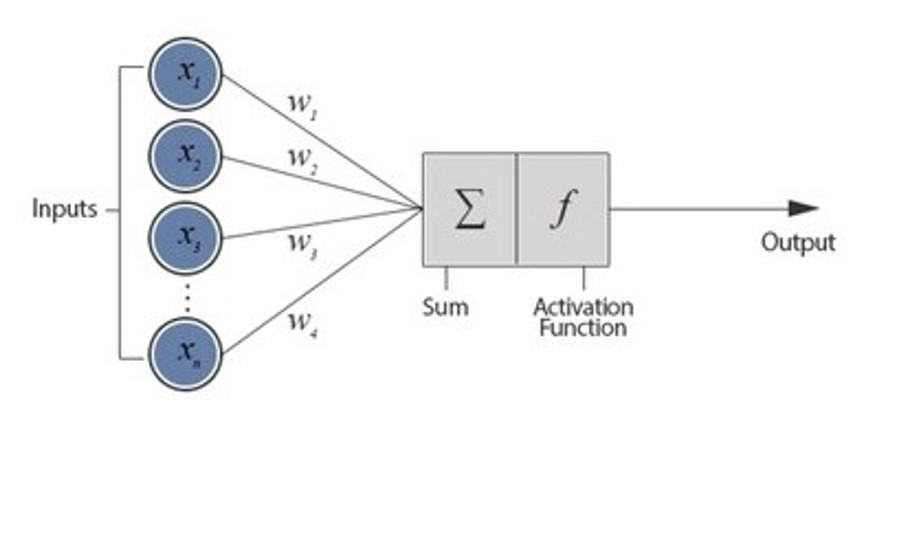
\includegraphics[width = 0.4\textwidth]{Images/nn_neuron}
		\label{fig:neuron}

	}
	
\end{figure}


For classification problems, the output layer typically uses a softmax function for multi-class problems to output a probability distribution over the classes, or a sigmoid function for binary classification problems to provide the probability of the positive class \cite{goodfellow2016deep}.




Training a neural network involves a two-step process: \textit{forward propagation} and \textit{backpropagation}. \\

In \textbf{forward propagation}, the input is passed through the network to generate an output. This output is then compared with the actual target to compute the loss function $ L $.

\textbf{Backpropagation} uses the chain rule of calculus to compute the gradient of $ L $ with respect to the network's parameters, which are then used to update the weights and biases:

\[
\frac{\partial L}{\partial w} = \frac{\partial L}{\partial a} \frac{\partial a}{\partial z} \frac{\partial z}{\partial w}
\]

Here, $ \frac{\partial L}{\partial a} $ is the derivative of the loss function with respect to the activation output, $ \frac{\partial a}{\partial z} $ is the derivative of the activation function, and $ \frac{\partial z}{\partial w} $ is the derivative of the weighted sum with respect to the weights.

Once these gradients are calculated, they are used to update the weights and biases via \textit{gradient descent}, an iterative optimization algorithm for finding the minimum of a function, in this case, the loss function. It is important to note that gradient descent is just one of many optimization techniques that can be used for this purpose, but it is widely used due to its efficiency and simplicity. This process iteratively adjusts the parameters to minimize the loss function \cite{ruder2016overview}:

\[
w_{\text{new}} = w_{\text{old}} - \alpha \frac{\partial L}{\partial w}
\]

\[
b_{\text{new}} = b_{\text{old}} - \alpha \frac{\partial L}{\partial b}
\]

In these equations, $ \alpha $ is the learning rate, a hyperparameter that determines the size of the steps the algorithm takes down the gradient towards the minimum.

The interconnected structure of ANNs, combined with the ability of backpropagation and gradient descent to effectively adjust the model parameters, allows these networks to learn and represent complex, non-linear relationships, in the data.
